\chapter{MULTILAYER DRIPPING HANDRAIL}
\thispagestyle{empty}

\mquote{The universe doesn't care if we understand it.}{Honey Badger Ph.D.}

Accretion disc model developed for the purpose of this study is composed of $n$ times $m$ individual cells arranged in concentric circular grid, where $n$ is the number of concentric layers and $m$ number of cells in its layers.

Each cell holds a set of parameters and its behaviour is governed by set of ordinary differential equations derived from MSMM \footnote{Defined in section \ref{section:msm}.}, so fundamentally every cell is its own \emph{dripping faucet}. Layers move in the same direction\footnote{Direction is arbitrary and a matter of perspective (i.e. top vs. bottom view).} with Keplerian orbital velocities relative to the outermost layer, which move by exactly one cell angular length in one simulation step. In every simulation step, there is a predefined constant mass influx into the outermost layer. This influx could come from specific azimuth or it could be distributed in some probabilistic manner from a wider range of angels.

As the simulation progresses, the mass is distributed in tangential direction by the orbital movement of layers and in radial direction by overflow from individual cells. This radial mass transfer is unidirectional towards the grid center and is triggered by a critical condition of MSMM in specific cells. 

Cell parameters and radial mass overflow are logged separately and later used to compute the radiative output, which is strongly dependent on radial mass transfer through changes in cell temperature and energy losses in gravitational potential of the imagined central body. 

Based on its characteristics, this model is called a \emph{Multilayer Dripping Handrail} and hereinafter it shall be referenced as MDH.

\section{MDH grid structure}

The cells are arranged in concentric circular grid of $n$ layers and $m$ cells in each layer. Layers are denoted by $i \in [0, n-1]$, with the outermost layer having the index $i = 0$. Individual cells in each layer are denoted by $j \in [0, m-1]$\footnote{Direction of $j$ index iteration is arbitrary and depends on implementation.}. Figure \ref{fig:grid_states} shows simplified representation of this concentric simulation grid in a) its initial state and b) in shifted state after arbitrary number of simulation steps. 

\begin{figure}
\centering
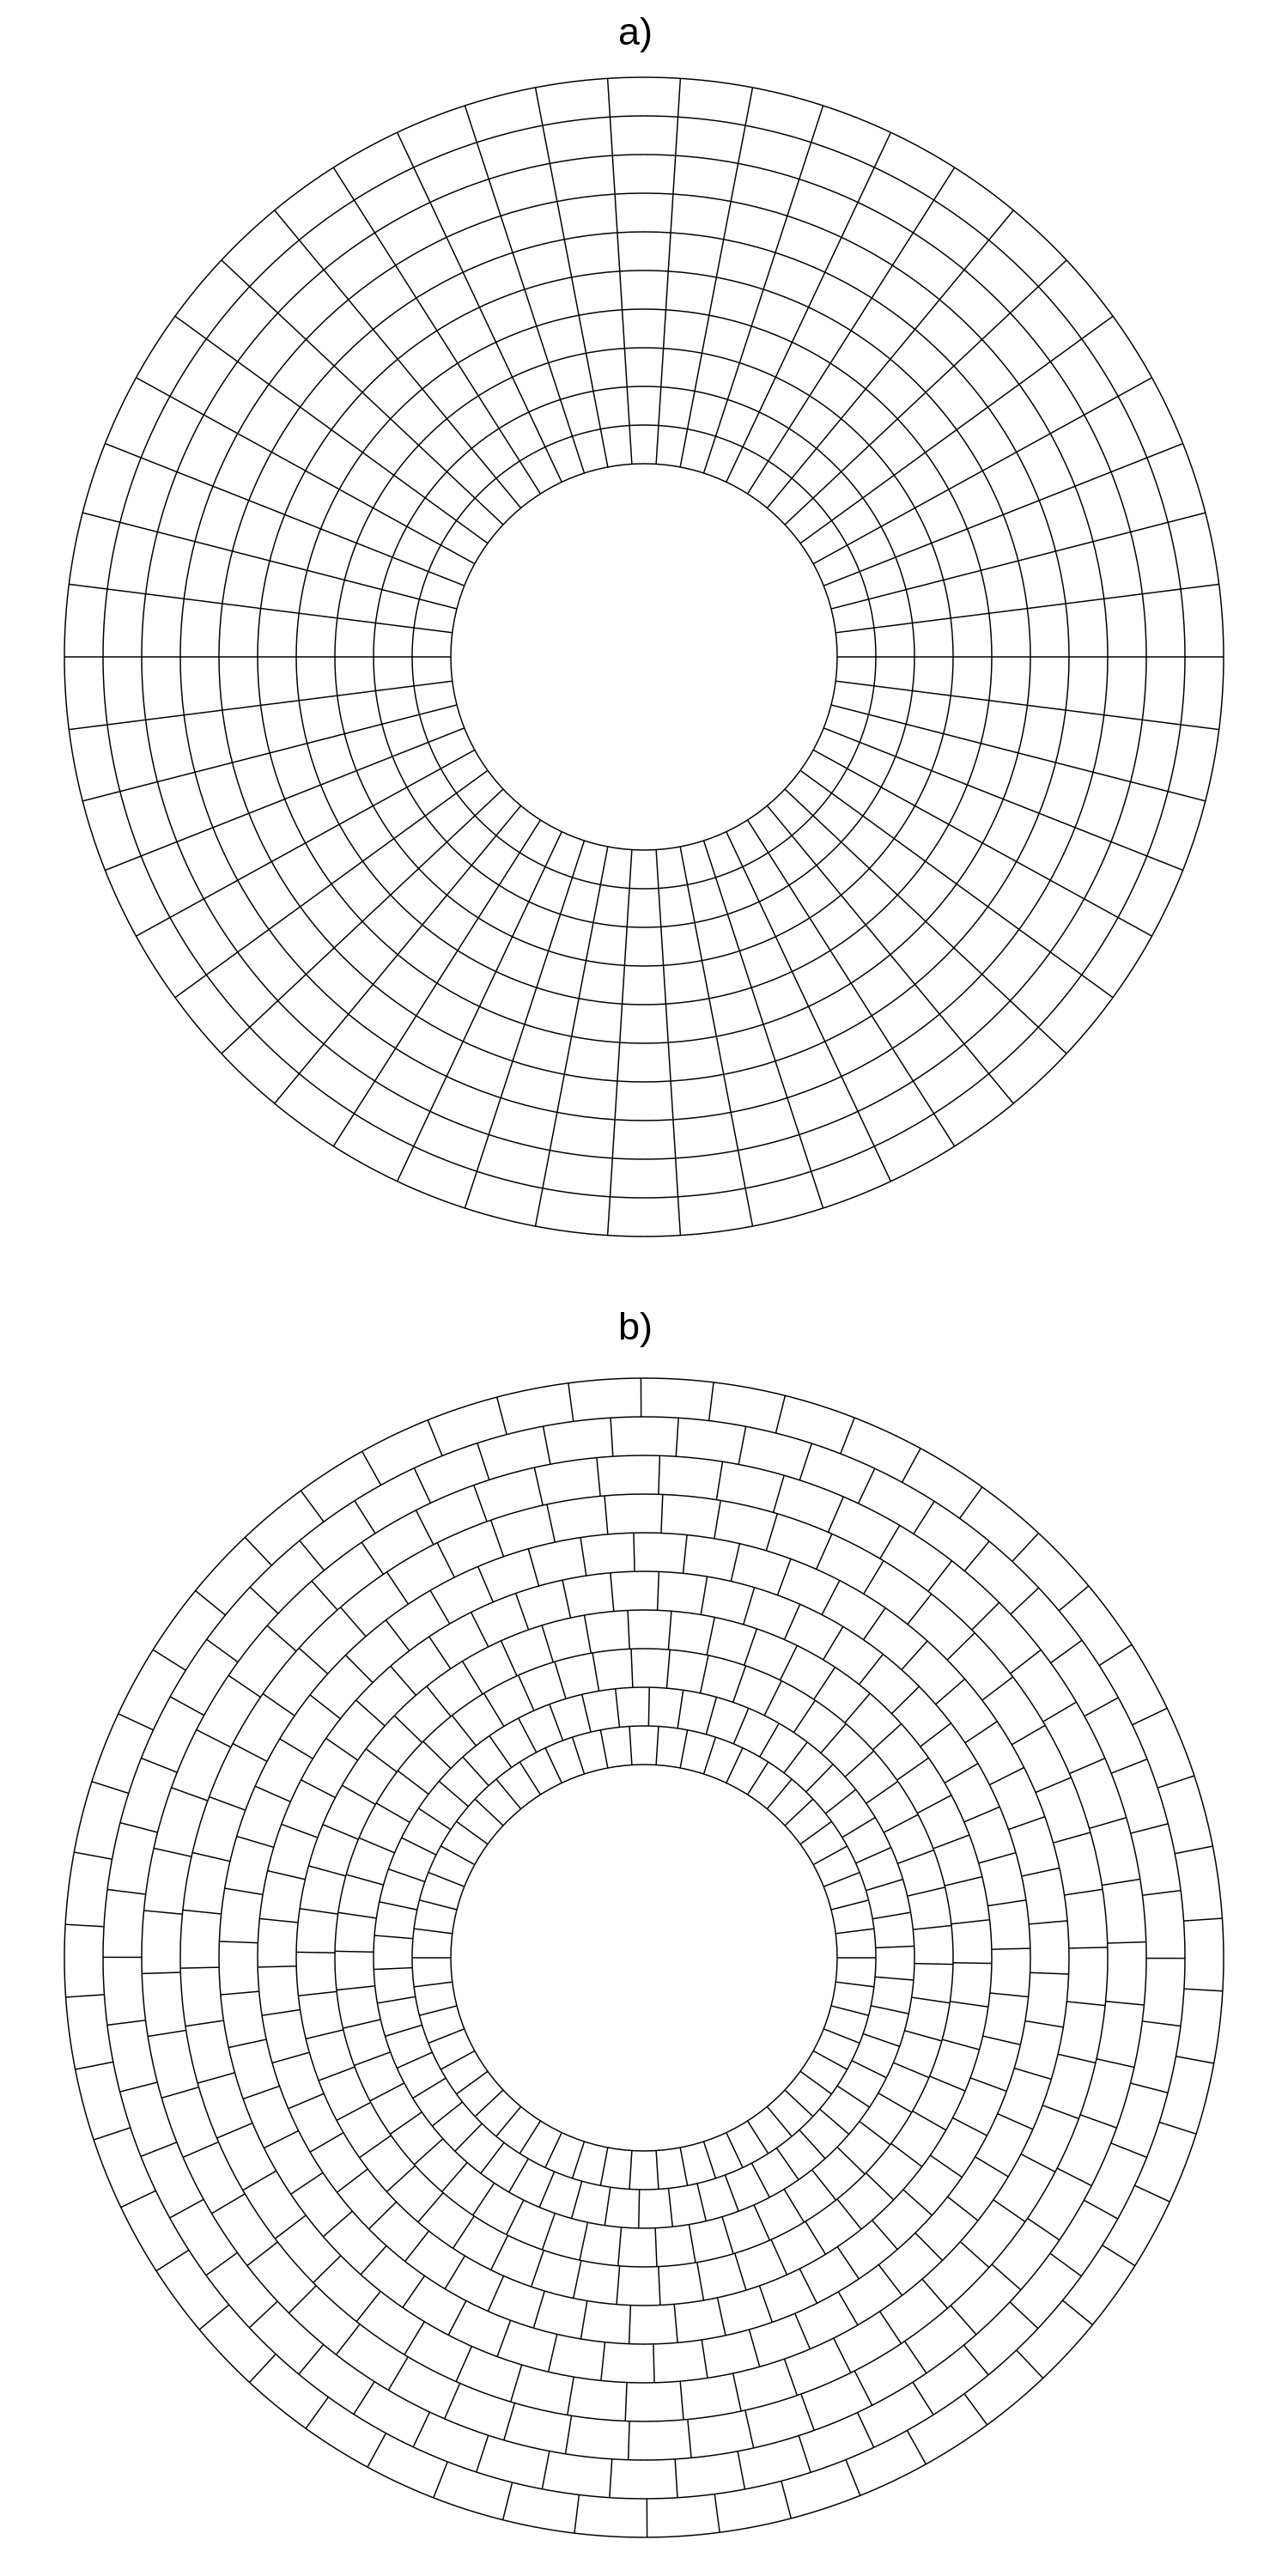
\includegraphics[width=0.75\columnwidth]{img/grid_states.png}
\caption{Simulation grid states: a) Initial unshifted state b) Shifted state after arbitrary number of simulation steps}
\label{fig:grid_states}
\end{figure}

Whole simulation grid acts like a cellular automaton (CA). Cellular automata models usually implement some kind of simple condition or set of conditions (e.g. Conway's game of life, see \cite{gardner1970}), to decide simulation development for the next step. In the case of model created by \cite{yonehara1997}, there is a simple mass limit condition to trigger the radial mass transfer. MDH takes this concept further and implements the condition as critical value of \emph{spring elongation} $z$ of MSMM, which is the solution of its ODE system solved in every simulation step. 

\section{Cell definition}
Individual cells are defined by a set of parameters. These parameters are listed in table \ref{table:mdh_cell_parameters} and following sections discuss some of them in detail.

\begin{table}[h]
\begin{center}
\begin{tabular}{r|l}
$i$			& Layer index \\
$j$			& Cell index \\
$r$			& Orbital radius \\
$\theta$	& Orbital azimuth \\ 
$f_g$		& Gravitational acceleration relative to outermost layer \\
$z$			& MSMM \emph{spring elongation}  \\
$v$			& MSMM \emph{velocity} \\
$m$			& Mass contained within the cell \\
$\Delta m$ 	& Mass change since previous step \\
$\gamma$		& Constant MSMM dampening parameter \\
$k$			& MSMM \emph{spring stiffness} \\
$T$			& Cell temperature
\end{tabular}
\caption{MDH model cell parameters}
\label{table:mdh_cell_parameters}
\end{center}
\end{table}

\subsection{MDH model geometry}
Position and size of specific cell in MDH model is derived from real world geometry of modelled accretion disc system. Parameters in question, are the orbital radius $r$ and orbital azimuth $\theta$. To define the orbital radius $r$, first the inner $r_{in}$ and outer $r_{out}$ radii of the accretion disc must be defined. The modelled system is considered to be a typical CV star\footnote{MDH can be modified to be applicable to other types of accreting systems.}, therefore in the first approximation $r_{in}$, that defines the boundary layer between accretion disc and central body, is set to be equal to the radius of the white dwarf. Using the \emph{White Dwarf Mass-Radius Relationship} it can be estimated, that radius is inversely proportional to the cube root of white dwarfs mass (citace!!):

\begin{equation}
    r_{in} \sim M_p^{-1/3},
\end{equation}

\begin{equation}
	r_{in} = 2 \cdot 10^{4} \left(\frac{\beta}{0.5}\right)^{5/3} \left(\frac{M_p}{M_{\odot}}\right)^{-1/3},
\end{equation}

where $M_p$ represents mass of the white dwarf and $\beta$ is ??? . Outer radius $r_{out}$ represents the outer edge of accretion disc, that is constrained by the Roche potential (citace!!!). Outer radius $r_{out}$ is then calculated as:

\begin{equation}
    r_{out} = d \cdot \frac{M_{s}}{3 \cdot (M_p+M_{s})^{1/3}},
\end{equation}

where $d$ represents the distance between binary system components and $M_s$ represents mass of the secondary donor star. Space between $r_{in}$ and $r_{out}$ is discretize into regularly spaced intervals according to chosen radial dimension $n$:

\begin{equation} \label{eq:cell_radius}
    r_i = r_{in} + (n - i - 1) \cdot \frac{r_{out} - r_{in}}{n - 1},
\end{equation}

\subsection{Azimuth and angular velocity profile}
Accretion disc layers (i.e. rings) are divided into equally spaced $m$ number of cells. Angular position is expressed by its orbital azimuth $\theta \in [0, 2\pi]$. Because orbits are considered to be Keplerian, and for simplicity circular, layers move at differing angular velocities. MDH model defines, that the outermost layer $i = 0$ moves by exactly one \emph{cell angular length} in one simulation step. Which means, that the cell azimuth change $d\theta$ in one step is:

\begin{equation} \label{eq:outer_azm_change}
d\theta(0) = \frac{2\pi}{m},
\end{equation}

where $m$ is the number of cells in one layer. The \emph{angular velocity profile} $f_{\omega}(i)$ is defined to describe the movement of any layer relative to the outermost layer $i=0$: 

\begin{equation} \label{eq:azm_profile}
f_{\omega}(i) = \frac{\omega_i}{\omega_0},
\end{equation}

where $\omega_0$ is the angular velocity of layer $i=0$. Angular velocity of any layer is calculated as: 

\begin{equation} \label{eq:omega_i}
\omega_i = \frac{v_i}{r_i},
\end{equation}

where $v_i$ represents the orbital velocity and $r_i$ is result of equation \ref{eq:cell_radius}. The cell orbital velocity $v_i$ is:

\begin{equation} \label{eq:velocity_i}
v_i = \sqrt{\frac{G \cdot M_p}{r_i}}.
\end{equation}

Combining equations \ref{eq:outer_azm_change} and \ref{eq:azm_profile} yield the azimuth change $d\theta$ in one simulation step for cells in any layer:

\begin{equation} \label{eq:azm_change}
d\theta(i) = \frac{\omega_i}{\omega_0} \cdot \frac{2\pi}{m}.
\end{equation}

Substitution of equations \ref{eq:velocity_i} and \ref{eq:omega_i} into equation \ref{eq:azm_change} cancels out the $\sqrt{GM_p}$ term and gives the final form of layer specific azimuth change in one simulation step:

\begin{equation} \label{eq:azm_change_final}
d\theta(i) = \left(\frac{r_{0}}{r_i}\right)^{3/2} \cdot \frac{2\pi}{m} = \left(\frac{r_{out}}{r_i}\right)^{3/2} \cdot \frac{2\pi}{m}.
\end{equation}

Equation \ref{eq:azm_change_final} is a discrete description of orbital movement of MDH cells, and therefore the mass contained within, for any modelled cell. Figure \ref{fig:profile_omega} shows such angular velocity profile $f_{\omega}(i)$ for specific system and its geometry.

\begin{figure}[H]
\centering
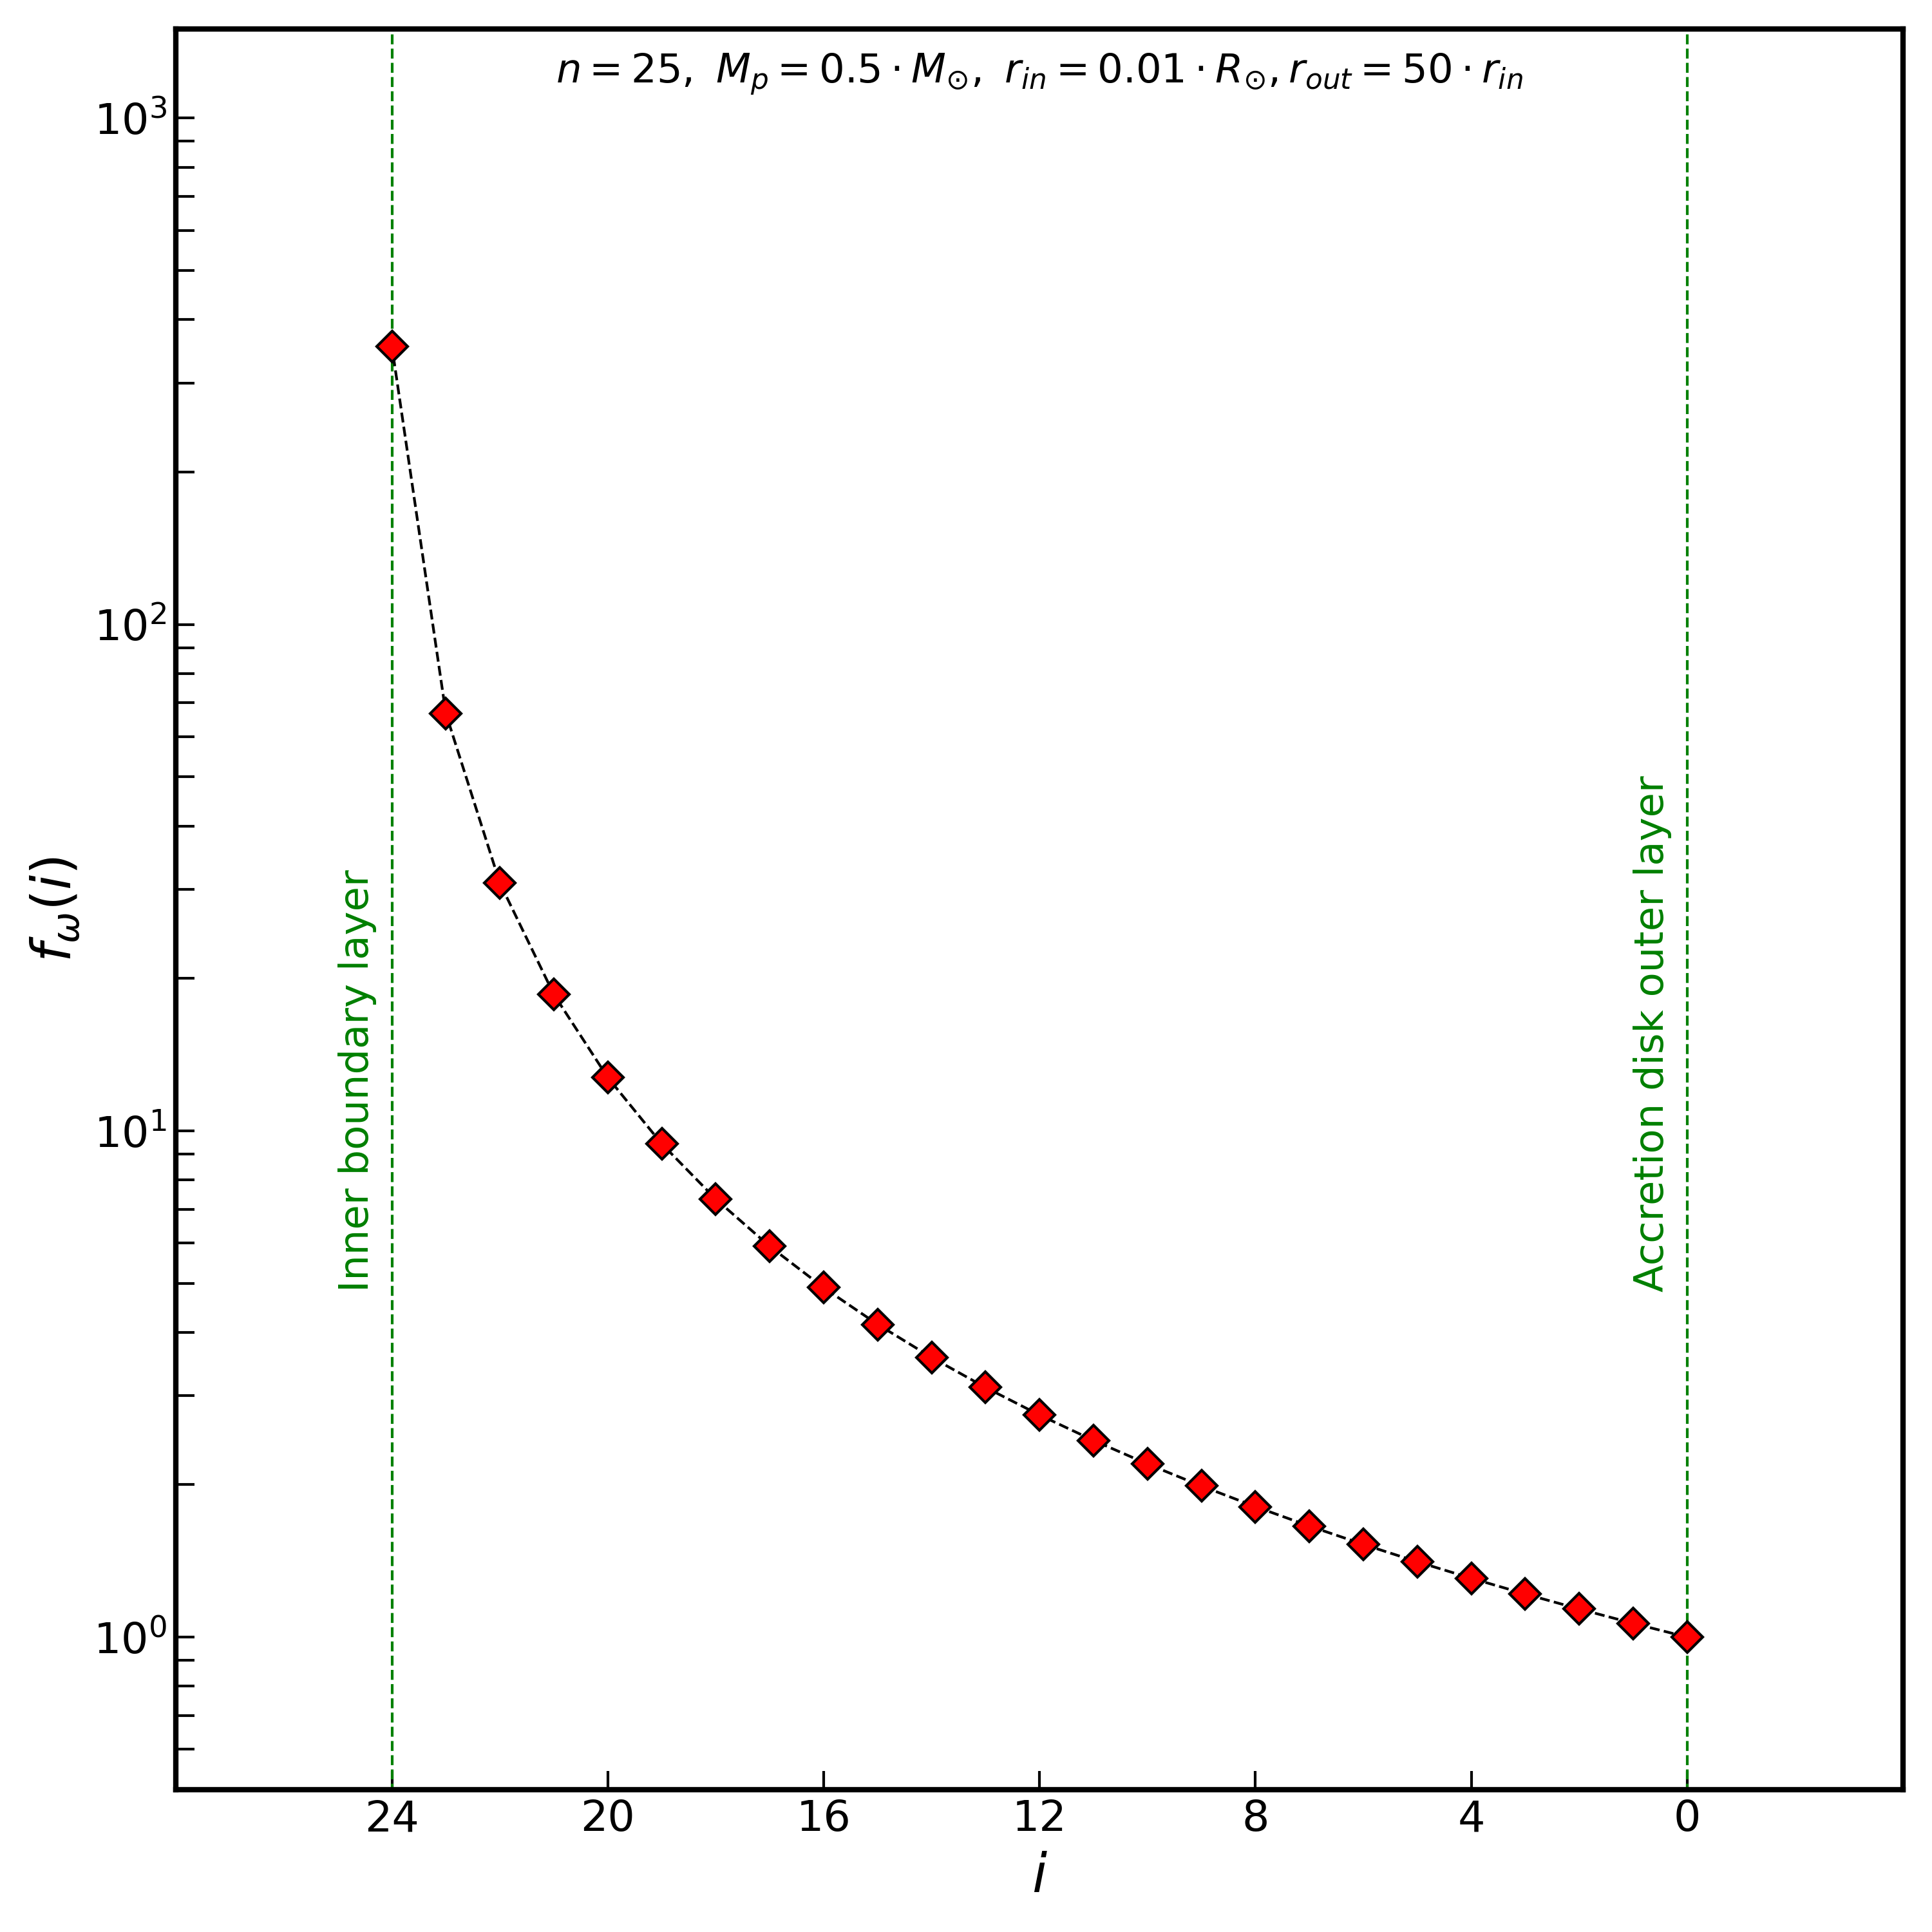
\includegraphics[width=0.9\columnwidth]{img/profile_omega.png}
\caption{Angular velocity profile relative to the layer $i = 0$ with modelled system parameters: $n=25$, $M_p = 0.5 \cdot M_{\odot}$, $r_{in} = 0.01 \cdot R_{\odot}$, $r_{out} = 50 \cdot r_{in}$}
\label{fig:profile_omega}
\end{figure}

\subsection{Gravity profile}

Similarly to angular velocity profile $f_{\omega}(i)$, the MDH model defines gravity profile $f_g(i)$, because the value of gravitational acceleration $g$ may differ by few orders of magnitude between central and outer regions of the accretion disc.  Value of $g_i$ for specific layer is:

\begin{equation} \label{eq:layer_g}
g_{i} = \frac{GM_{p}}{r_{i}^2},
\end{equation}

where $M_p$ represents mass of the central object, $G$ is the universal gravitational constant and $r_i$ is layer radius (i.e. distance to the center of gravity). Same as in the case of angular velocity profile $f_{\omega}(i)$ the gravity profile $f_g(i)$ is defined as relative value to the outermost layer $i = 0$ as:

\begin{equation} \label{eq:profile_g}
f_g(i) = \frac{g_i}{g_0}
\end{equation}

Substitution of equation \ref{eq:layer_g} into \ref{eq:profile_g} cancels out again the $GM_p$ term and gives the final form of gravity profile:

\begin{equation} \label{eq:profile_g_final}
f_g(i) = \left(\frac{r_{0}}{r_i}\right)^2=\left(\frac{r_{out}}{r_i}\right)^2.
\end{equation}

Figure \ref{fig:profile_g} shows example of such a profile and results of equation \ref{eq:profile_g_final} are later used in cell MSMM ODE system to describe the differing influence of central object on mass in specific cells. 

\begin{figure}[H]
\centering
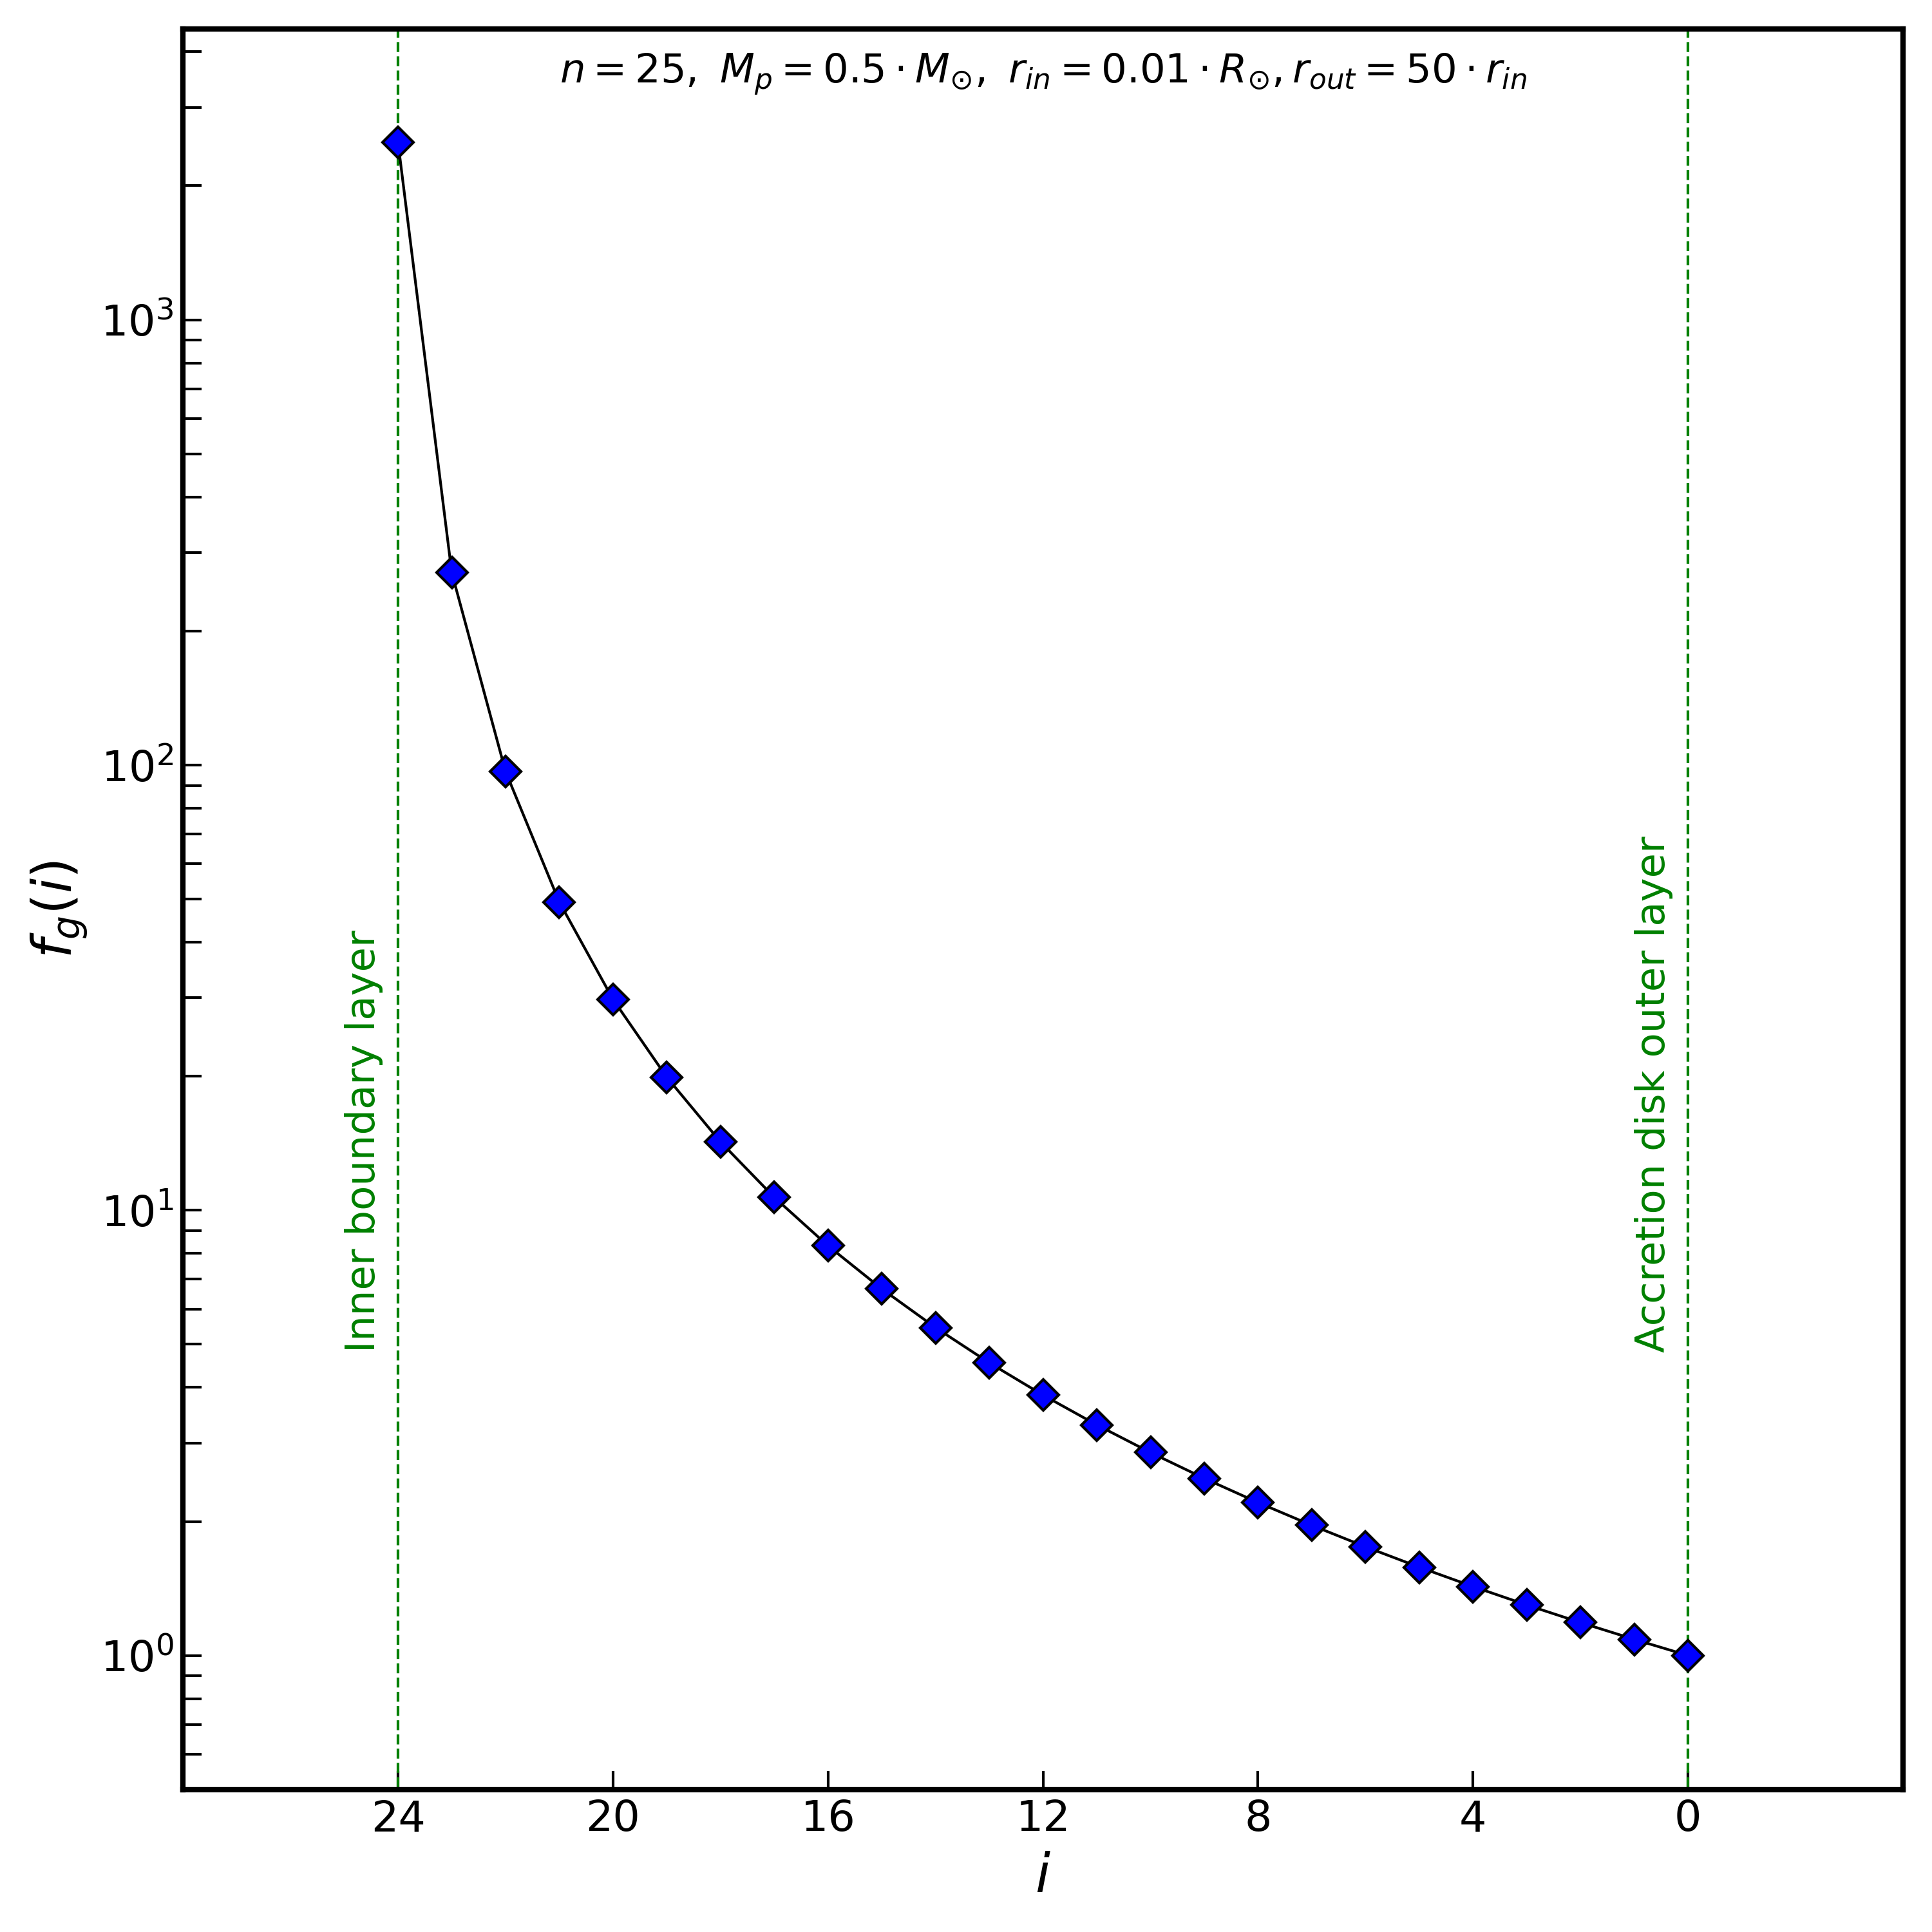
\includegraphics[width=0.9\columnwidth]{img/profile_g.png}
\caption{Gravity profile relative to the layer $i = 0$ with modelled system parameters: $n=25$, $M_p = 0.5 \cdot M_{\odot}$, $r_{in} = 0.01 \cdot R_{\odot}$, $r_{out} = 50 \cdot r_{in}$}
\label{fig:profile_g}
\end{figure}

\subsection{MSMM parameters}



MSMM ODE system ... 

\begin{equation}
    \D{}{t} \left(m \D{z}{t}\right) = -kz - \gamma\D{z}{t} + f_g(i) \cdot m,
\end{equation}
\begin{equation}
    \D{m}{t} = Q = const.,
\end{equation}

MSMM \emph{spring stiffness} ...

\begin{equation}
    \begin{aligned}
        & k~= 
        \begin{cases}
            -11{,}4m + 52{,}5 \hspace{10mm} (m < 4{,}61) \\
            \hspace{10mm} 0 \hspace{21mm} (m \ge 4{,}61 ),
        \end{cases}
    \end{aligned}
\end{equation}

Mass redistribution criteria ...

\begin{equation}
    m_r = 0.2m+0.3.
\end{equation}

\subsection{Temperature}

\section{Simulation}

Layer orbital period ...

\begin{equation}
    T_{i=0} = \sqrt{\frac{4 \pi^2 r_{out}^3}{G M_{p}}}.
\end{equation}

Time step size ...

\begin{equation}
    h = T_{i=0} / m,
\end{equation}



